\chapter{Variational Mixture of Normalizing Flows}
\label{chapter:vmonf}

\section{Introduction}
\label{section:vmonf-intro}

As mentioned in sections \ref{section:probmodellatvar} and \ref{section:mmodels},
the ability of leveraging domain knowledge to endow a probabilistic model with
structure is often useful. The goal of this work is to devise a model that combines
the flexibility of normalizing flows with the ability to exploit class-membership
structure. This is achieved by learning a mixture of normalizing flows, via
optimization of a variational objective, for which the variational posterior
over the class-indexing latent variables is parameterized by a neural network.
Intuitively, this neural network should learn to place similar instances of
data in the same class, allowing each component of the mixture to be fitted
to a cluster of data.

\section{Model Definition}

Let us define a mixture model as in section \ref{section:mmodels}, where each of
the $K$ components is a normalizing flow. For simplicity, consider that all of
the $K$ normalizing flows have the same architecture\footnote{This is not a requirement,
and in cases where we have classes with different levels of complexity, we can
have components with different architectures. However, the training procedure
does not guarantee that that the most flexible normalizing flow is "allocated"
to the most complex cluster. This is definitely an interesting direction for future
research.}, i.e., they are all composed of the same stack of transformations,
but they each have their own parameters.

Additionally, let $q(z|\bm{x};\gamma)$ be a neural network with a softmax output, with
parameters $\bm\gamma$. This network will receive as input an instance from the
data, and produce the probability of that instance belonging to each of the
$K$ classes.

Recall the evidence lower bound given in \ref{eq:elbokldiv}\footnote{Here the
dependence of $q$ on $x$ is made explicit}:
\begin{equation*}
    \text{ELBO} = \mathbb{E}_q [\log p(\bm{x}, z)] - \mathbb{E}_q [\log q(z|\bm{x})]
\end{equation*}

Let us rearrange it:
\begin{align}
    \text{ELBO} &= \mathbb{E}_q [\log p(\bm{x}|z)] + \mathbb{E}_q [\log p(z)] - \mathbb{E}_q [\log q(z|\bm{x})]
        \label{eq:threepartelbo} \\
    &= \mathbb{E}_q [\log p(\bm{x}|z) + \log p(z) - \log q(z|\bm{x})] \label{eq:simplerelbo}
\end{align}

Since $q(z|\bm{x})$ is given by the forward-pass of a neural network, and is therefore
straightforward to obtain, the expectation in \ref{eq:simplerelbo} is given by
computing the expression inside the expectation for each possible value of $z$,
and summing the obtained values, weighed by the probabilities given by the variational posterior.
Thus, the whole ELBO is easy to compute, provided that each of the terms inside
the expectation is itself easy to compute. Let us consider each of those terms:
\begin{itemize}
    \item $\log p(\bm{x}|z)$ is the log-likelihood of $\bm{x}$ under the normalizing
        flow indexed by $z$. It was shown in the previous chapter how to compute
        this.
    \item $\log p(z)$ is the log-prior of the component weights. For simplicity,
        let us assume this is set by the modeller. When nothing is known about
        the component weights, the best assumption is that they are uniform.
        Nevertheless, as will be shown empirically, this too can be optimized.
    \item $- \log q(z|\bm{x})$ is the negative logarithm of the output of the encoder.
\end{itemize}

For a better intuition about each of these terms, it is useful to review the last
paragraph of the first subsection of Section \ref{subsubsection:kldiv}.

Let us call this model Variational Mixture of Normalizing Flows (VMoNF). For an overview of
the model, consider figures \ref{fig:plate} and \ref{fig:modeloverview}

\begin{figure}[!htb]
  \centering
  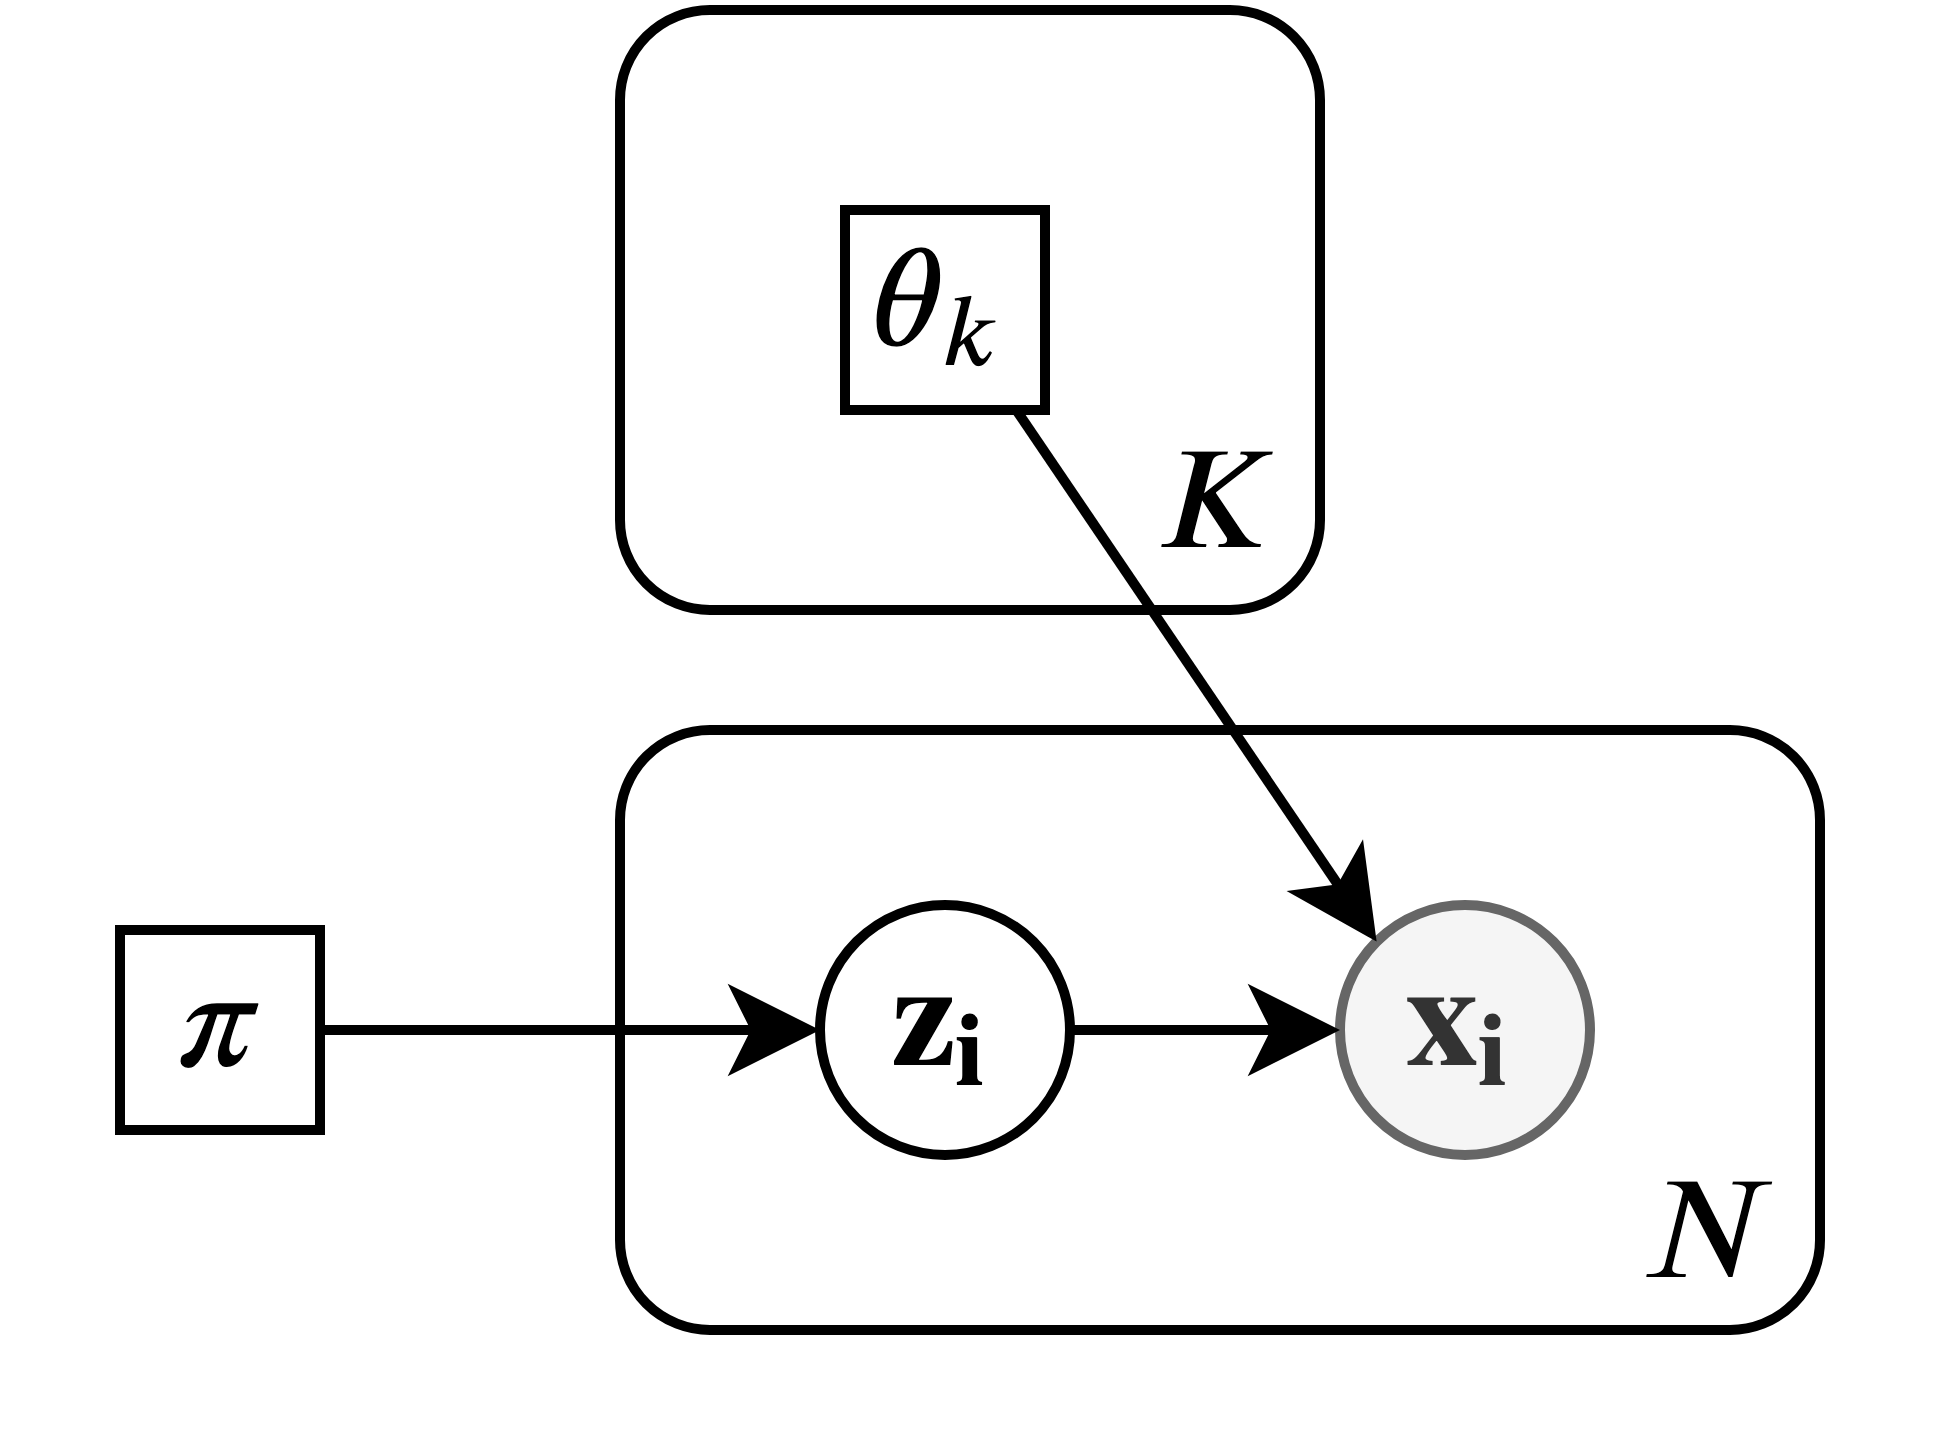
\includegraphics[width=0.5\linewidth]{figures/plate_diagram.png}
  \caption{Plate diagram of a Mixture of $K$ Normalizing Flows. $\bm\theta_k$ is the
    parameter vector of component $k$.}
  \label{fig:plate}
\end{figure}

\begin{figure}[!htb]
  \centering
  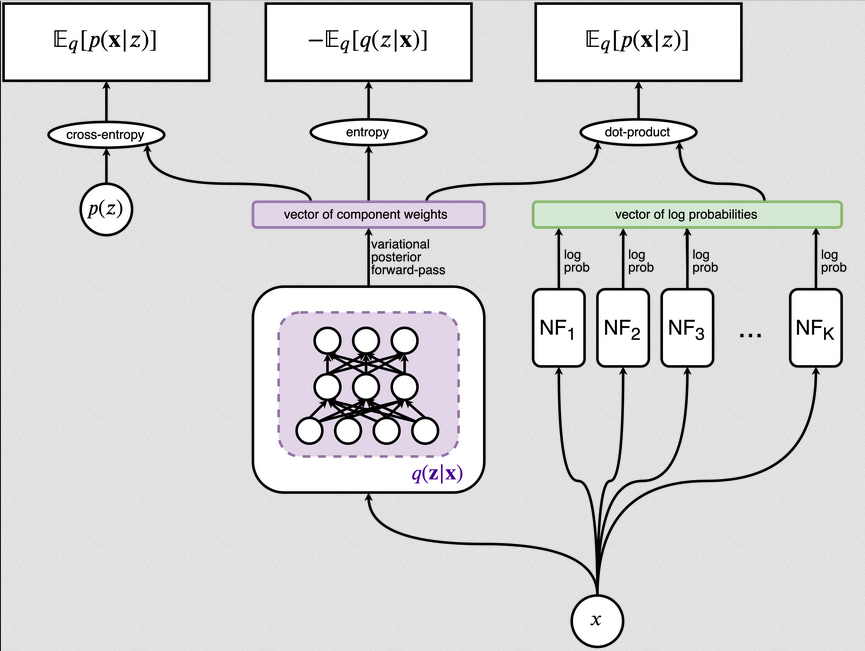
\includegraphics[width=0.85\linewidth]{figures/train_overview.png}
  \caption{Overview of the training procedure.}
  \label{fig:modeloverview}
\end{figure}

In a similar fashion to the Variational Auto-Encoder, proposed in \autocite{vaepaper},
a VMoNF is fitted by jointly optimizing the parameters of the variational
posterior $q(z|\bm{x}; \bm\gamma)$ and the parameters of the generative process
$p(\bm{x}|z; \bm\theta)$.

After training, the variational posterior can be directly used as a classifier
for new data points, as will be shown in the experiments section.

\section{Implementation}

To implement and test the proposed model, Python was the chosen language. More
specifically, this work heavily realies on the PyTorch (\autocite{pytorch}) package
and framework for automatic differentiation. Moreover, the parameter optimization
is done via stochastic optimization, namely using the optimizer proposed in
\cite{adam} - Adam.

Figure \ref{fig:modeloverview} gives an overview of the training procedure:
\begin{enumerate}
    \item The \emph{log-probabilities} given by each component of the mixture
    are computed.
    \item The values of the variational posterior probabilities for each
    component are computed.
    \item With the results of the previous steps, all three terms of the ELBO
    are computable.
    \item The ELBO and its gradients w.r.t the model parameters are computed
    and the parameters are updated.
    \item Steps 1 to 4 are repeated until some stopping criterion is met.
\end{enumerate}

